\chapter{Experimentos y resultados}

Se realizaron 2 tipos de experimentos: de visión y de manipulación. Pruebas de resolución no se llevaron a cabo, ya que el solucionador siempre encuentra una solución, a menos que el cubo se encuentre en un estado inválido.

Se utilizó el scrambler legacy de la World Cube Association, el generador que solía utilizarse en las competencias oficiales de speedcubing para permutar  cubos. Con él se generaron $20$ permutaciones del cubo de Rubik. Cada una de estas permutaciones, también llamados ``desarmes'', consiste de $30$ rotaciones, y fueron aplicadas manualmente sobre el cubo. La tabla \ref{vision} del apéndice muestra las secuencias de rotaciones utilizadas en cada experimento.

\section{Visión}
Para la visión, se utilizaron los $20$ desarmes en su totalidad. Cada ejecución comenzó con el robot recogiendo el cubo desde una mesa.

\begin{figure}[h!]
	\centering
	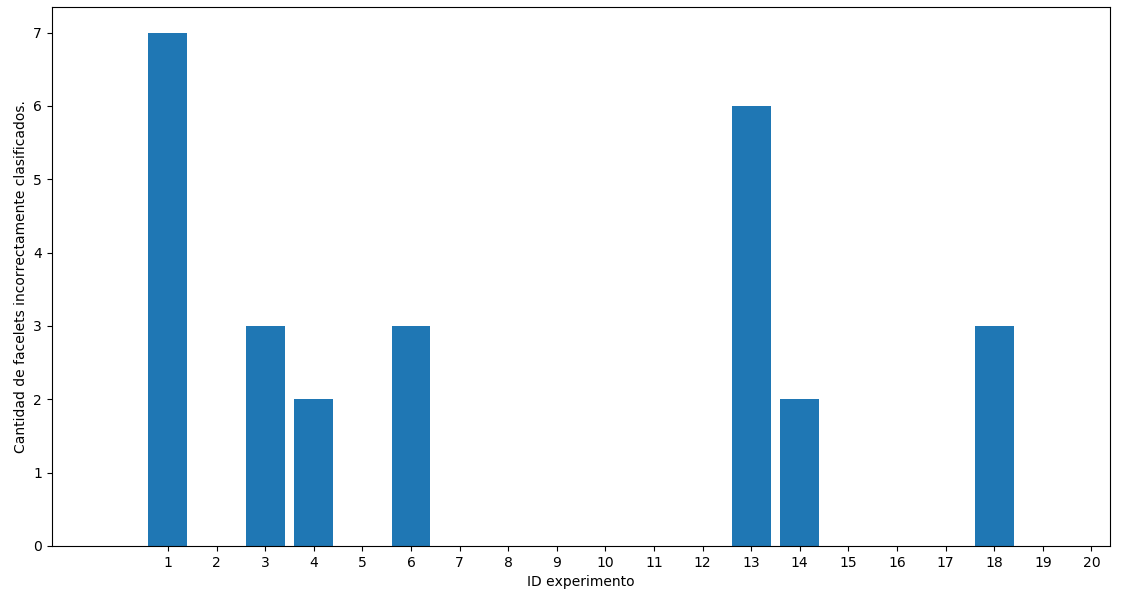
\includegraphics[width=\textwidth]{figures/error_facelet}
	\caption{Facelets mal clasificados por cada prueba realizada.}
	\label{erroresfacelets}
\end{figure}
Del total de pruebas, el 65\% no tuvo errores de clasificación. La cantidad de facelets mal clasificados en promedio fue de $1.35$ facelets, con desviación estándar de $2.220$. La cantidad de facelets mal clasificados en cada experimento se muestra en la figura \ref{erroresfacelets}. En la tabla \ref{visionerrors} del apéndice, se muestra específicamente cuales fueron los estados del cubo en cada ejecución, y exactamente cúales fueron los faceles indebidamente clasificados.

Respecto a la totalidad de facelets en todos los experimentos, el $97.5$\% fue etiquetado correctamente. Lamentablemente, basta con 1 sólo facelet incorrecto para que el solver sea incapaz de encontrar una solución, por lo que en el mejor de los casos el robot hubiese sido capaz de resolver el $65$\% de estos desarmes.

\begin{figure}[h!]
	\centering
	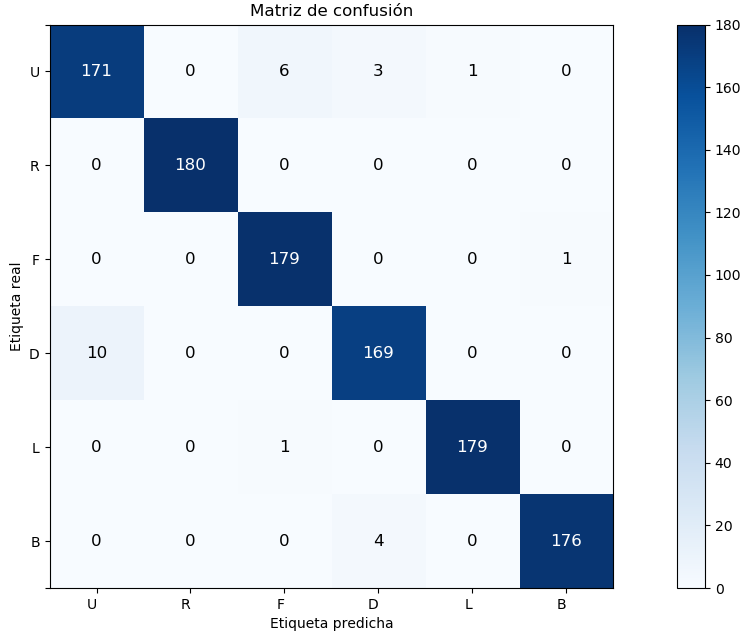
\includegraphics[width=0.7\textwidth]{figures/conf_matrix}
	\caption{Matriz de confusión de predicción de colores, sin normalizar.}
	\label{confusion}
\end{figure}
\begin{figure}[h!]
	\centering
	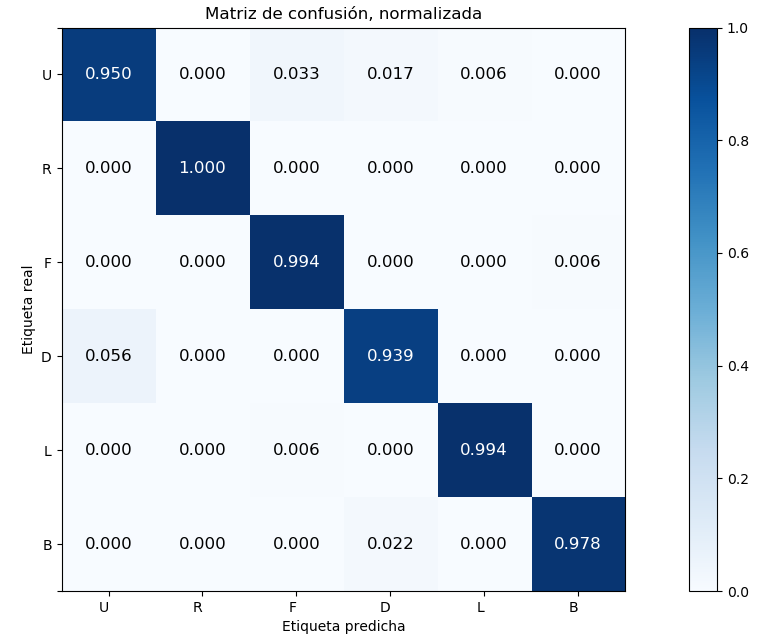
\includegraphics[width=0.7\textwidth]{figures/conf_matrix_norm}
	\caption{Matriz de confusión de predicción de colores, normalizada.}
	\label{confusionnorm}
\end{figure}

Una parte importante de los errores se dieron entre las caras U y D, que en las pruebas realizadas correspondieron a los colores rojo y rosado. Estos colores son muy similares entre sí, aunque esto depende mucho de las condiciones de iluminación del ambiente donde se encuentre el robot. El detalle de los errores por cara se muestra en las figuras \ref{confusion} y \ref{confusionnorm}.



\section{Manipulación}
Para esta clase de pruebas se utilizaron los mismos desarmes que en las pruebas de visión, pero con el desarme $i$ truncado a $i$ rotaciones. De esta manera, se probó una secuencia por cada uno de los largos de secuencias posibles, desde el mínimo ($1$) hasta el máximo ($20$). Se midió en cuál giro el robot es incapaz de proseguir. Los resultados se ven en la tabla \ref{resultadogiros}.

\begin{table}[h!]
	\centering
	\begin{tabular}{|r|r|l|}
		\hline
		Largo & Cambios & Resultado \\ \hline \hline
		 1 & 1 & Ejecución completada exitosamente \\ \hline
		 2 & 0 & Ejecución completada exitosamente \\ \hline
		 3 & 1 & Ejecución falla en giro 3 \\ \hline
		 4 & 2 & Ejecución completada exitosamente \\ \hline
		 5 & 2 & Ejecución completada exitosamente \\ \hline
		 6 & 1 & Ejecución completada exitosamente \\ \hline
		 7 & 4 & Ejecución completada exitosamente \\ \hline
		 8 & 2 & Ejecución completada exitosamente \\ \hline
		 9 & 5 & Ejecución falla en giro 6 \\ \hline
		10 & 5 & Ejecución completada exitosamente \\ \hline
		11 & 7 & Ejecución completada exitosamente \\ \hline
		12 & 8 & Ejecución falla en giro 8 \\ \hline
		13 & 10 & Ejecución falla en giro 3 \\ \hline
		14 & 10 & Ejecución falla en giro 4 \\ \hline
		15 & 6 & Ejecución falla en giro 14 \\ \hline
		16 & 8 & Ejecución falla en giro 5 \\ \hline
		17 & 10 & Ejecución falla en giro 10 \\ \hline
		18 & 10 & Ejecución falla en giro 14 \\ \hline
		19 & 11 & Ejecución falla en giro 12 \\ \hline
		20 & 12 & Ejecución falla en giro 8 \\ \hline
	\end{tabular}
	\caption{Resultados experimentos de manipulación. La columna ``largo'' es el largo de la secuencia y la columna ``cambios'' es la cantidad de cambios de mano que debe realizar el robot para ejecutarla.}
	\label{resultadogiros}
\end{table}

\begin{figure}[h!]
	\centering
	\includegraphics[width=\textwidth]{figures/cambios_corr}
	\caption{Cantidad de cambios de mano versus fracción de la secuencia ejecutada correctamente.}
	\label{corr}
\end{figure}
Si se observa la figura \ref{corr}, se nota que a medida que aumenta la cantidad de cambios de mano, disminuye la fracción de la secuencia ejecutada exitosamente, aunque con gran variabilidad. Si notamos que a medida que crece el largo de una secuencia es más probable que hayan más cambios de mano, esto explica el por qué los desarmes más largos nunca fueron ejecutados en su totalidad. No obstante, esto no quiere decir que las secuencias cortas o con pocos cambios de mano estén libres de errores. Obsérvese por ejemplo, el caso de la secuencia $3$. A pesar de consistir de tan solo $3$ movimientos y $1$ cambio de mano, el robot fue incapaz de llevar a cabo la secuencia en su totalidad, fallando en el último giro. En el otro extremo se presentan casos como el de la secuencia $11$, que con $11$ movimientos y $7$ cambios de mano se pudo ejecutar por completo.

Otra de las causas de error en la manipulación se deben a la precisión del robot Baxter. Sus especificaciones indican un error de $\pm 0.5$ centímetros al controlar las posiciones de las pinzas. Los facelets del cubo de Rubik utilizado tiene un ancho de $1.83$ centímetros, por lo que hay poco margen para los errores de precisión de hardware. Los fallos generados al acumular errores luego de varias rotaciones dentro de una misma secuencia se pueden clasificar en los siguientes tipos:
\begin{enumerate}
	\item agarre muy profundo: el robot intenta girar con un gripper una cara bloqueada por el otro brazo, produciendo que piezas aristas o esquinas salgan disparadas.
	\item agarre poco profundo: el robot intenta girar con un gripper una cara pero no consigue estar lo suficientemente cerca. Esto no maltrata el cubo, pero produce que todas las rotaciones posteriores lleven el cubo a un estado totalmente distinto del deseado.
	\item cambio de mano mal alineado: al cambiar el cubo de un gripper a otro, se bloquea accidentalmente alguna o varias de las caras que debiesen quedar libres. Esto puede permitir la ejecución momentáneamente, dependiendo de los giros siguientes, pero eventualmente puede causar errores del tipo $1$ o $2$.
\end{enumerate}

Respecto de la visión, el factor más importante al detectar los colores correctamente es la iluminación. Aún con el cubo cubierto con goma EVA, el sólo hecho de apuntar el cubo en ángulos distintos hacia la cámara produce varianzas importantes entre los puntos representantes de un mismo color. Debido a los límites de las articulaciones del robot, no fue posible hacer que para las caras \emph{U} y \emph{D} (las que quedan opuestas a las cámaras de los brazos del robot) quedasen perfectamente perpendiculares a la cámara de la cabeza robot. Para compensar este hecho, se le dio un ángulo de inclinación a las demás caras, pero que nuevamente, por limitaciones en las articulaciones del robot no fue exactamente el mismo ángulo que para las caras \emph{U} y \emph{D}. Esta pequeña diferencia se puede apreciar en las figuras \ref{gmmgood} y \ref{gmmbad}, donde se ve que cada color esta formado por 2 sub clusters. En cada cluster, el sub cluster de más arriba (es decir, el con mayor saturación), corresponde a facelets en las caras \emph{U} y \emph{D}, que recibieron mayor luz al estar ligeramente más inclinados hacia la fuente de luz de la habitación. Si bien se podrían evitar las inclinaciones en ángulos distintos al agregar cambios de mano adicionales (para que las caras U y D no queden opuestas a las mano del robot), esto incurriría en más acumulación de errores de precisión, además de romper los invariantes definidos y aumentar la cantidad de posturas, complejizando bastante la manipulación y ralentizando la ejecución.

% Necesario?
Para finalizar, no se consideran los resultados presentados (por ``buenos'' que hayan sido) como indiscutibles, pues dado que la magnitud del espacio de estados del cubo de Rubik es enorme ($\approx 4.5\times 10^{19}$), ninguna cantidad no descomunal de pruebas será representativa de todas las configuraciones posibles.
